\documentclass[11pt,border=2pt]{standalone}
\usepackage{amsmath,amssymb}
\usepackage{xcolor}
\usepackage{tikz}
\usepackage{pgfplots}
\pgfplotsset{compat=1.18}
\usetikzlibrary{calc,arrows,positioning,fit,backgrounds,decorations.pathreplacing,patterns}
\definecolor{cElem}{RGB}{40,80,140}
\definecolor{cTrg}{RGB}{190,40,40}
\definecolor{cCell}{RGB}{225,238,248}
\definecolor{cAcc}{RGB}{240,200,120}
\definecolor{cGrey}{RGB}{120,120,120}
\definecolor{cVec}{RGB}{110,55,150}
\begin{document}
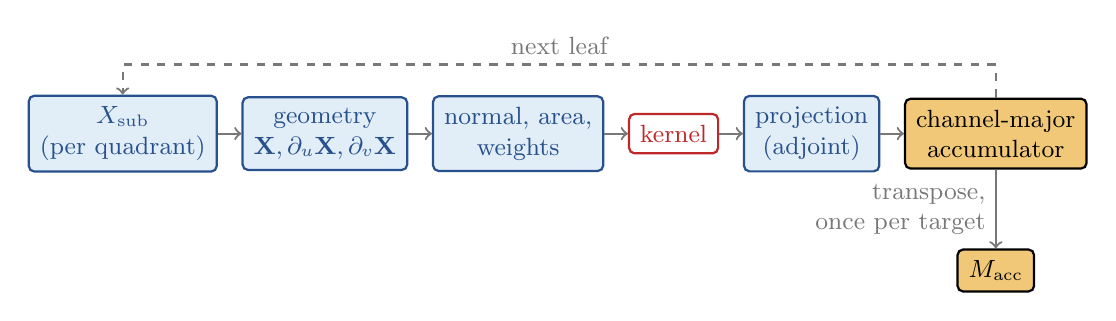
\begin{tikzpicture}[node distance=3mm,
   b/.style={draw,cElem,thick,fill=cCell,rounded corners=2pt,align=center,inner sep=4pt,font=\small},
   k/.style={draw,cTrg,thick,fill=white,rounded corners=2pt,align=center,inner sep=4pt,font=\small},
   o/.style={draw,thick,fill=cAcc,rounded corners=2pt,align=center,inner sep=4pt,font=\small},
   a/.style={->,thick,cGrey}]
  \node[b] (x)  {$X_{\text{sub}}$\\ (per quadrant)};
  \node[b,right=of x]  (gt) {geometry\\ $\mathbf{X},\partial_u\mathbf{X},\partial_v\mathbf{X}$};
  \node[b,right=of gt] (as) {normal, area,\\ weights};
  \node[k,right=of as] (kk) {kernel};
  \node[b,right=of kk] (pr) {projection\\ (adjoint)};
  \node[o,right=of pr] (ac) {channel-major\\ accumulator};
  \draw[a] (x)--(gt); \draw[a] (gt)--(as); \draw[a] (as)--(kk); \draw[a] (kk)--(pr); \draw[a] (pr)--(ac);
  \node[o,below=10mm of ac] (mm) {$M_{\text{acc}}$};
  \draw[a] (ac)--(mm) node[midway,left,align=right,font=\small] {transpose,\\once per target};
  \draw[a,dashed] (ac.north) -- ++(0,0.42) -| (x.north)
        node[pos=0.25,above,font=\small] {next leaf};
\end{tikzpicture}
\end{document}
